\documentclass[../main.tex]{subfiles}
\graphicspath{{\subfix{../images/}}}
\begin{document}

\subsection{Problem Definition}

Compilation can be understood in layman terms as a text-processing task, which 
takes sentences of computer code in a higher-level, more abstract language, into
equivalent sentences written in a lower-level, less abstract language. Decompilation
can be then understood as the inverse procedure: taking sentences written in a
lower-level language and writing equivalent sentences in a higher-level language.
An example is illustrated on figure \ref{fig:decompilation_example} 

\begin{figure}[htbp]
\centering
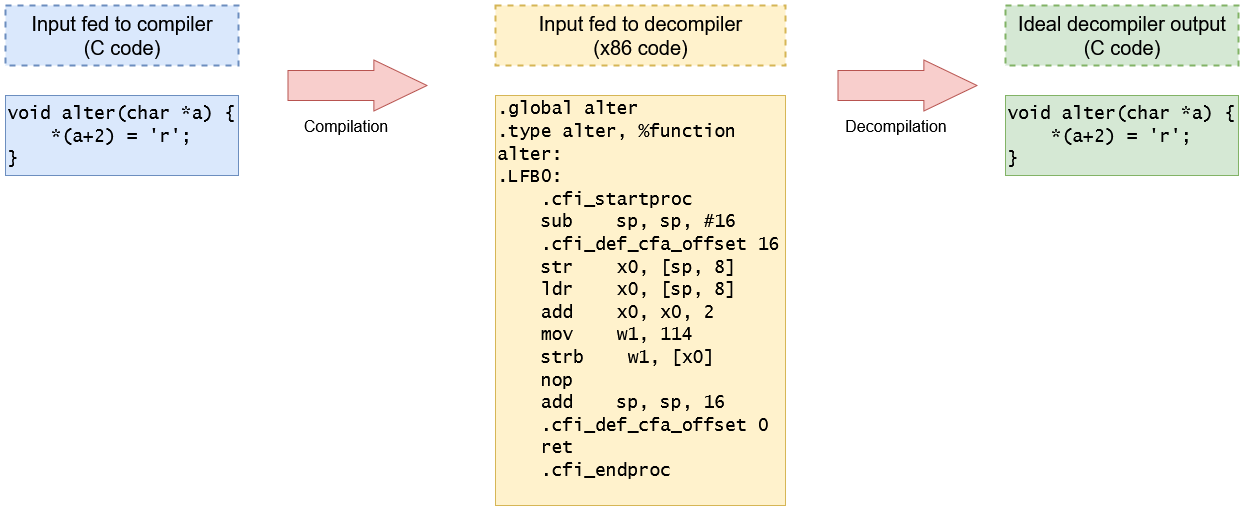
\includegraphics[width=0.5\textwidth]{images/decompilation_example.png}
\caption{Example of plausible input for decompiler, and ideal output}
\label{fig:decompilation_example}
\end{figure}

However, the decompilation task presumes the precedence of previous compilation: 
it's fundamentally more about the reversal of compilation than it is about
the swapping of roles of the origin and destination languages involved in the
presumed translation. This distinction comes into play when discussing the use
cases and applications of decompilation in industry; like for example. the case
of reverse engineering in cybersecurity applications \cite{lin_reverse_2010} \cite{durfina_design_2011}, which
main use case is understanding the underlying workings of malware. Similarly, on
software development portability efforts, it's easier to work with code written
on a higher-level language due to its legibility and closeness in abstractions to
the way people design software. 
Indeed, the goal is not merely to just end up with equivalent code in a higher-level
language, but rather to also have it resemble the human-friendly structures and
expressiveness that the original high-language source code — from which the low-level
code is presumed to have came from — had in the first place.

Plainly put, we try to tackle decompilation from low-level, x86 ISA assembly code (with
64-bit extensions) into legible, human-readible and standard-conforming conforming C
code (with no fixed standard), with a limited scope of single-source, single-destination
file decompilation. 

\subsection{Related Work}

\subsubsection{Common challenges}

Long before the introduction of Machine Learning approaches there were plenty of
techniques applied to decompilation in virtue of domain-specific knowledge. Most 
can be summarized into four main distinct phases: syntax analysis, semantic analysis,
data-flow analysis and control-flow analysis \cite{cifuentes_reverse_1994}, 
each of which had their own approaches, such as pattern matching, analysis of 
control-flow graphs, type inference, and many more.

Nevertheless, many problems arise when attempting decompilation. Some are listed
below as described by \cite[p.~1-7]{cifuentes_reverse_1994}:
\begin{itemize}
    \item \textit{Recursive Undecidability}: More often than not for high-level 
    languages, in the general case predicting which instructions may or may not 
    execute is undecidable, which makes difficult the separation of instruction from
    data on von Neumann architectures. 
    \item \textit{Self-modifying code}: Some programs benefit from the ability to
    modify their own instructions, like security-critical encripted programs or
    viruses. Anticipating the ways on which programs modify themselves before translation
    is commonly also undecidable.
    \item \textit{Architecture-dependent restrictions}: Some instructions carry
    operational semantics specific to some architectures, which require some degree
    of emulation to fully anticipate the effects of.
    \item \textit{Sub-routines included by the toolchain}: A great deal of instructions
    external to the main source code for a program are often required for it to be
    executable or functional at all. These routines can be embedded at compile-time
    or referenced and loaded at run-time. These dependencies are hard to account for,
    or decompile at all.
\end{itemize}

\subsubsection{Principled approaches}

Previous works on native x86 decompilation pre-existing the aid of Machine Learning
techniques have existed for a while. 
The Phoenix decompiler developed by \cite{brumley_native_2013} makes use of a novel
control-flow structuring algorithm that aims to produce functionally equivalent
high-level C-code from a binary source, on virtue of analyzing control-flow graphs.
Other intermediate representations distinct from control-flow graphs can also
often used: as demonstrated by \cite{van_emmerik_static_2007} by repurposing the 
Static-Single Assignment (SSA) form — commonly used in compiler optimization —
for decompilation analysis; and as demonstrated by \cite{durfina_design_2011} by 
translation to intermediate LLVM IR code guided by encoding and semantics provided
by an ISAC model, an intermediate bridge for the operational semantics in assembly
back to a higher-level language. 

Other industry-ready compilers based upon expert domain-knowledge of specific 
programming languages exist already. IDA \cite{hexrays}, Ghidra \cite{ghidra}
and RetDec \cite{retdec} comprise some of the many examples freely-available. 
Nevertheless, they also suffer from poor readibility.

As showcased above, common theme in these approaches is the use of intermediate 
representations for the low-level code as a means of easier or richer analysis.
This pattern is not lost on further Machine Learning assisted techniques, which
attempt to exploit pre-existing relationships and structures — especially those
related to recursive relationships present in language — to more accurately
predict higher-level code with human-friendly readibility.

\subsubsection{Machine Learning approaches}

Machine Learning based approaches for decompilation often frame the problem as a 
text-processing problem; more specifically, as an instance of Neural Machine 
Translation (NMT). Thefore, the techniques employed are often borrowed from the
field of Natural Language Processing (NLP), and more often than not make use of
Sequence-to-Sequence (Seq2Seq) models \cite{DBLP:journals/corr/SutskeverVL14}

\cite{katz_using_2018} exemplified the use of Recurrent Neural Networks (RNNs) for 
binary-to-C decompilation, employing an encoder-decoder architecture. They first 
generate a corpus of C source-code data, which is then pre-processed into snippets
of Abstract Syntax Trees (ASTs) which are then compiled into binary-C pairs. The
pairs are tokenized and then fed into the model — C source code as inputs, binary 
as output — for training. Their tokenization scheme makes use of domain-knowledge 
analysis, and the training examples are bucketed according to length classes.
Their work demonstrated the potential efficacy of tackling decompilation as a NMT 
problem with the aid of RNNs. 

Multiple other studies share a similar approach, like \cite{hosseini_beyond_2022} 
which used a transformer-based, encoder-decoder architecture instead for a Seq2Seq
model.

\cite{katz_towards_2019} builds upon the work of \cite{katz_using_2018} and attempts 
to "compensate for the differences between natural languages and programming 
languages" by augmenting the decompilation process with programming-languages 
domain-knowledge. Their approach makes heavy use of canonicalization of assembly 
and C-source code, alongside the preservation of structure via template-filling. 
For templated-code generation, they made use of a modified version of a standard 
encoder-decoder, Attention-based, model architecture "DyNmt" \cite{dynmt}, and 
later compared the dependency graphs between the original source code and the 
predicted decompiled output.
\cite{liang_semantics-recovering_2021} similarly attempts to leverage the use of
intermediate representations of high-level and low-level code. They translated 
high-level code into an intermediate, serialized representation with embedded 
semantic information but removed from the syntax structure of the high-level 
language. This intermediate representation is not only directly convertible back
to the high-level code it was built from, but aids in compensating the information
asymmetry between the high-level and the low-level code while resembling the 
syntactic structure found in low-level code. Likewise, they use self-attention 
mechanisms on the underlying model architecture.
Both of these works expanded upon the NMT approach to decompilation by exploiting
structure of programming languages, and making use of intermediate representations
to aid in training Large Language Models (LLM)s.

\cite{fu_n-bref_2020} takes intermediate source code representation even further: 
by shifting the input and output spaces from texts to graphs they better account 
for the inherent structures in programming languages. Low-level code is represented 
as control/data flow graphs, while high-level source code is represented as ASTs.
The source-code ASTs are predicted via inductive Graph Neural Networks (GNNs).
Additionally, they split decompilation into sub-tasks: data-type resolution and 
source-code generation. The layers of their architecture are implemented by back-bone
structural transformers and self-attention modules.
Their work exemplifies the conceptual jump from framing decompilation purely as a
text-processing task to reframing it as a graph-to-graph translation task, which
in turn can be subdivided into mpre specialized subtasks on a pipeline.

Type inference as its own separate task is explored by \cite{escalada_improving_2021},
who try to predict the return type from functions constructed by decompilers with
the aid of many machine-learning models beyond LLMs. Their problem is framed as
multi-class classification, where the possible return types are the categories and
detected patterns in the code — detected with the aid of LLMs — are extracted features.

\cite{cao_boosting_2022} also tackles decompilation with the aid of intermediate
graph representation of the low-level binary code taken as input, and a custom
intermediate representation of the high-level C code as an output. Just like 
\cite{fu_n-bref_2020}, they make use of GNNs to better capture dependencies in 
data and control flow of low-level code, and then make use of Long-Short-Term-Memory
(LSTMs) layers with a global attention mechanism to output the intermediate high-level
code representation.  Their work additionally leverages domain-specific knowledge
to recover operands.

Due to time and logistic constraints, we opted to fine-tune causal, text-prediction
LLM pre-trained on conversational tasks. Therefore, we frame the decompilation task
as a question answering task. Further details are given on section \ref{methodology}.

\subsubsection{Efficacy measurements}

There have been multiple proposed metrics for evaluating compilation and decompilation
results, as well as code legibility. \cite{le_compiler_2014} proposed a methodology
for validating compiler outputs. Its underlying principle lies in "dynamically
executing a program on some test inputs", constructing a collection of variants
which can then be compared for two distinct compilers and a given source code.
Comparing these collections for equivalency can help find key differences in compiled
results across compilers.

The previous methodology could be repurposed in order to compare compiled outputs
for the same compiler but between a reference original source code, and a decompiled
output. Further reading on C code decompilation correctness is available on 
\cite{liu_how_2020}.

Semantic correctness is not the only metric one could take to measure the efficacy
of a decompiler. Code legibility is one of the key desired aspects that Machine
Learning approaches to decompilation attempt to tackle. \cite{eom_r2i_2024} proposes
their own quantifiable metric for code readibility, specifically regarding the
decompilation results of popular decompilers.

Automated approaches to measuring the efficacy of LLMs decompiling C code have also
gone underway. \cite{vaaden_using_2024} showcases a simple pipeline for generating
pairwise examples of C and assembly code, generating decompiled outputs with both 
LLMs and common domain-knowledge, classic decompilers, and lastly evaluating their
results. Their main metric for evaluating readibility and correctness is CodeBLEU, a
composite metric \cite{ren2020codebleumethodautomaticevaluation} which combines the
scores of the traditional BLEU metric, AST and data-flow matching scores, to better
capture the structural and legibility similarities between the reference and generated
high-level code.

Due to time and logistic constraints, we developed recall, precision, $f_1$, 
perplexity and categorical cross-entropy loss measurements. Further details are
given on section \ref{methodology}.

\end{document}